\section{实验结果与分析}

\subsection{三种方法求解速度比较}

训练数据量$N = 10$,多项式次数$m = 3$,惩罚项系数$\lambda = 0$时,分别采用解析解法、梯度下降法、共轭梯度法进行多项式系数$w$的求解。拟合情况如图\ref{methods}。

\begin{figure}[htbp]
    \centering
    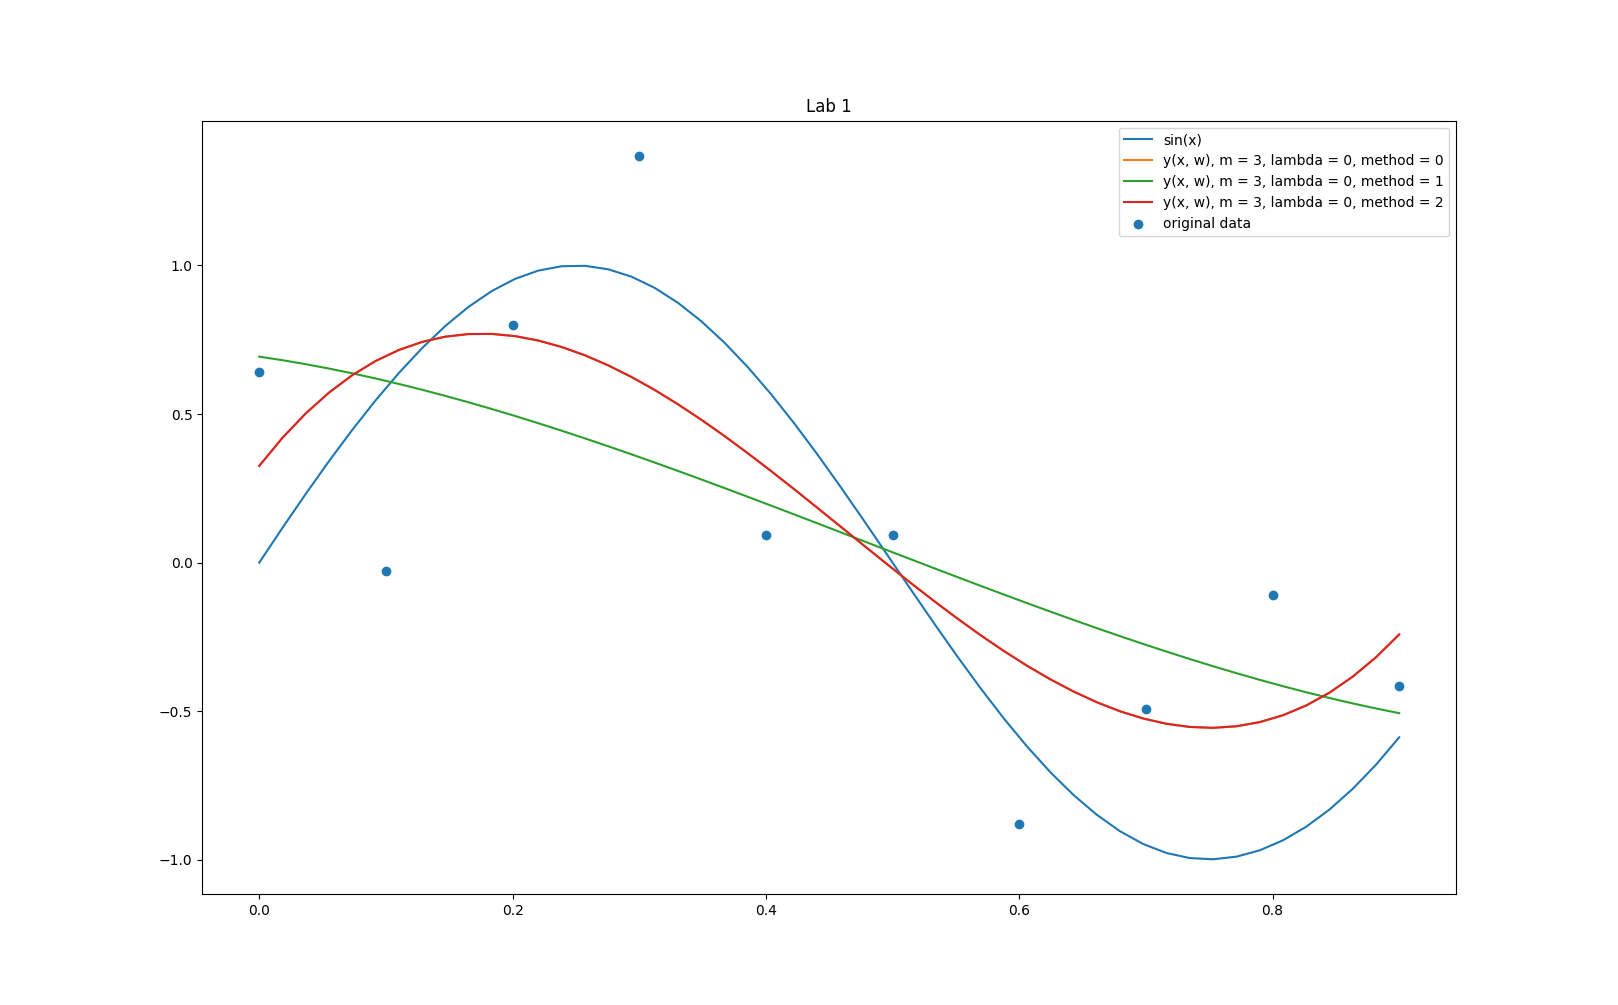
\includegraphics[width=0.7\textwidth]{figures/Figure_11.png}
    \caption{三种方法求解$w$。其中梯度下降法学习率$\alpha = 0.01$,迭代次数为$10000$次;共轭梯度法迭代次数为$10$次}
    \label{methods}
\end{figure}

可以看到,虽然共轭梯度法的迭代次数仅有梯度下降法的$\frac{1}{1000}$,但前者的效果仍然远优于后者。而后者的拟合效果已经和解析解法相差无几。

增加梯度下降法的迭代次数,如图\ref{methods1}。

\begin{figure}[htbp]
    \centering
    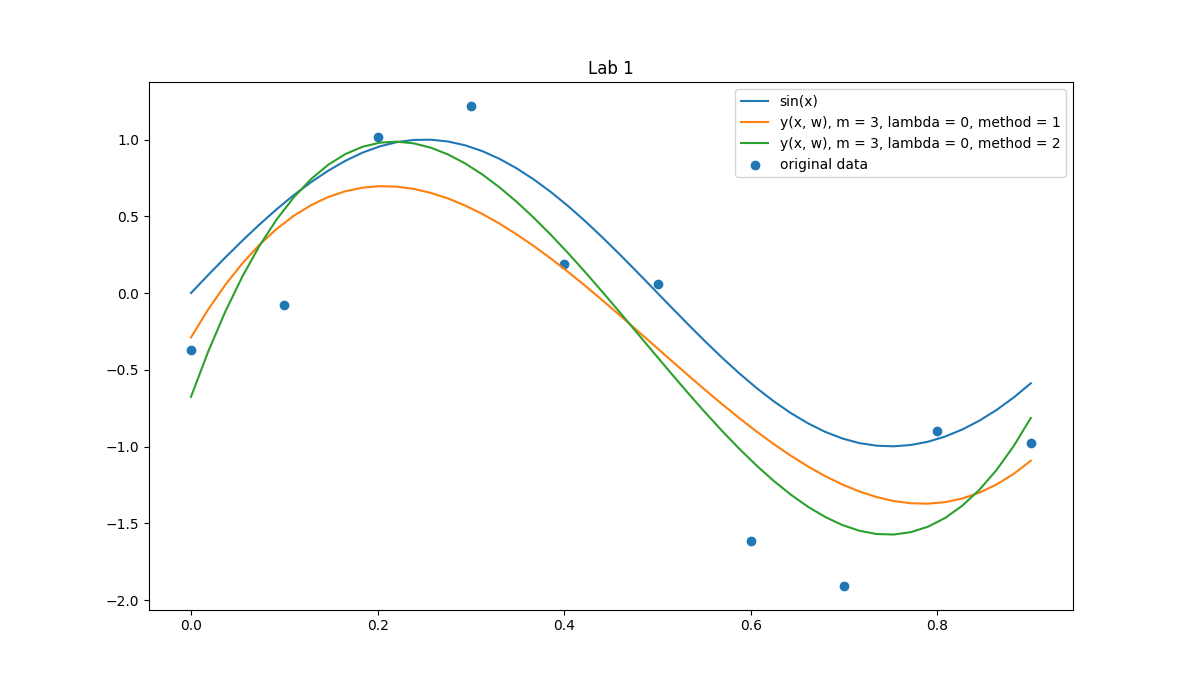
\includegraphics[width=0.7\textwidth]{figures/Figure_12.png}
    \caption{增加梯度下降法的迭代次数为$100000$次}
    \label{methods1}
\end{figure}

可以看到,当梯度下降法的迭代次数是共轭梯度法的$\frac{10000}{1}$时,二者才有相似的拟合效果。但梯度下降法所用的时间已经远远超出共轭梯度法所用时间。

所以,可以看出共轭梯度法收敛快、准确率高的优势,但是由于其只能够解决系数矩阵为对称正定矩阵的线性方程组$A x = b$的数值解的方法,故并不能普遍适用。

\subsection{无惩罚项}

\subsubsection{仅调整多项式系数}

调整训练数据量$N = 10$。当$m = 3, 5$时,拟合情况如图\ref{m3}和图\ref{m5}。

\begin{figure}[htbp]
    \begin{minipage}[t]{0.5\linewidth}
        \centering
        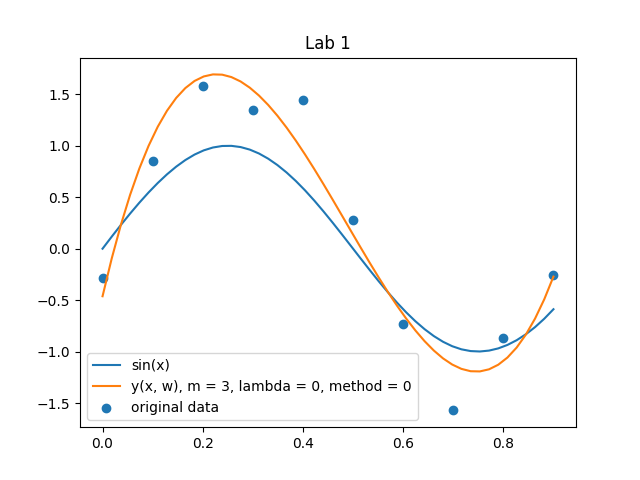
\includegraphics[width=\textwidth]{figures/Figure_2.png}
        \caption{$m = 3$时的拟合情况}
        \label{m3}
    \end{minipage}
    \begin{minipage}[t]{0.5\linewidth}
        \centering
        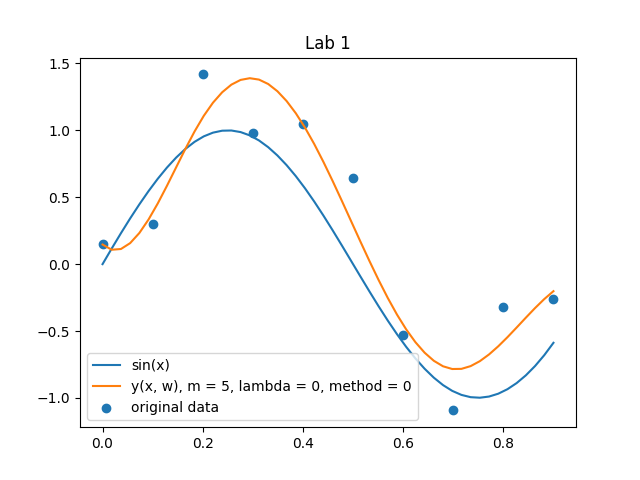
\includegraphics[width=\textwidth]{figures/Figure_3.png}
        \caption{$m = 5$时的拟合情况}
        \label{m5}
    \end{minipage}
\end{figure}

$m = 9$时,拟合情况如图\ref{m9}。

\begin{figure}[htbp]
    \centering
    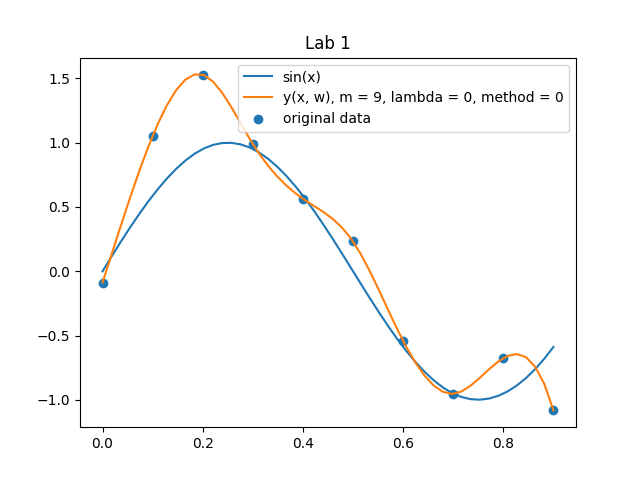
\includegraphics[width=0.7\textwidth]{figures/Figure_4.png}
    \caption{$m = 9$时的拟合情况}
    \label{m9}
\end{figure}

可以看到,在多项式阶数$m = 3$时的拟合效果已经很好。继续提高多项式的阶数,在阶数$m = 9$此时多项式曲线经过了每一个数据点(因为数据集一共有$N = 10$个点),但曲线已经严重变形,将所有噪声均很好的拟合,无法对将来的数据$x_n$进行预判。这种现象称为过拟合。

过拟合的本质是,在阶数过大的情况下,求解系数$w$时有唯一解,此解刚好可以穿过所有样本点。

可以通过增加样本的数据或者通过增加惩罚项的方式来解决过拟合问题。

计算$m = 2, 3, 4, ... 9$时,多项式函数拟合的误差,结果如图\ref{mn}

\begin{figure}[htbp]
    \centering
    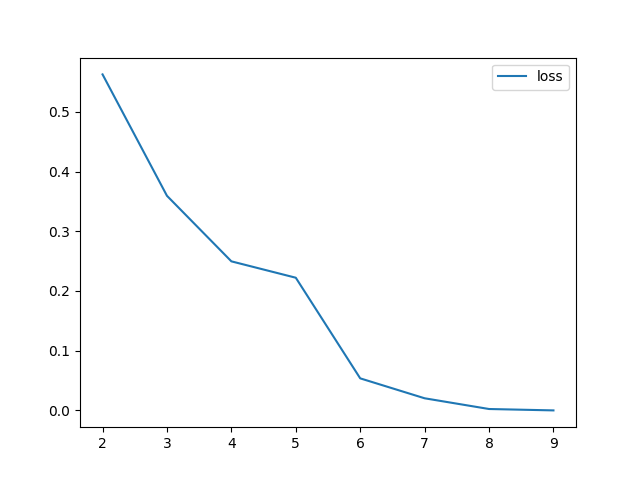
\includegraphics[width=0.7\textwidth]{figures/Figure_13.png}
    \caption{$m = 2, 3, 4, ... 9$时,多项式函数拟合的误差}
    \label{mn}
\end{figure}

可见当多项式次数$m$增加时,拟合效果逐渐变好。但是当重新生成测试数据时,获得的拟合效果误差如图\ref{mn2}。

\begin{figure}[htbp]
    \centering
    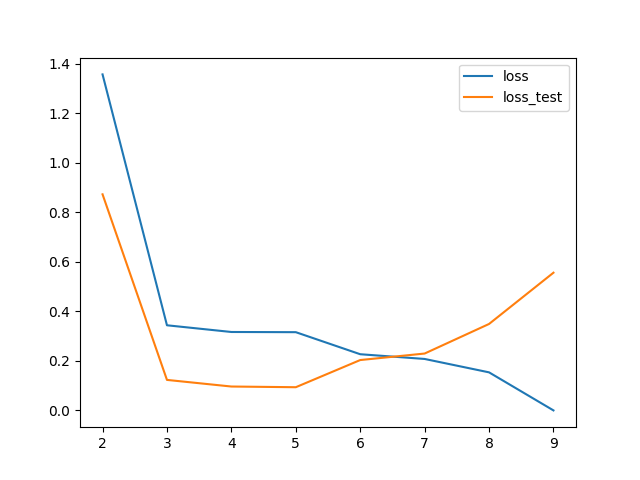
\includegraphics[width=0.7\textwidth]{figures/Figure_14.png}
    \caption{$m = 2, 3, 4, ... 9$时,重新生成测试数据后,多项式函数拟合的误差}
    \label{mn2}
\end{figure}

可见当多项式次数$m$增加时,测试数据的拟合效果不增反降。这个事实反映了过拟合现象的问题,即对于训练样本拟合效果太好,以致于对新的测试样本解释效果太差。

\subsubsection{仅调整数据量}

多项式函数次数$m = 9$时,调整数据量。当$N = 10, 20, 100, 1000$时的拟合情况如图\ref{N10}、\ref{N20}、\ref{N100}、\ref{N1000}。

\begin{figure}[htbp]
    \begin{minipage}[t]{0.5\linewidth}
        \centering
        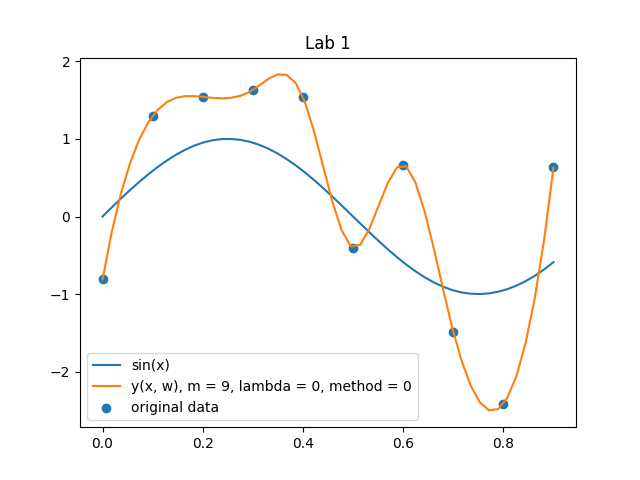
\includegraphics[width=\textwidth]{figures/Figure_5.png}
        \caption{$N = 10$时的拟合情况}
        \label{N10}
    \end{minipage}
    \begin{minipage}[t]{0.5\linewidth}
        \centering
        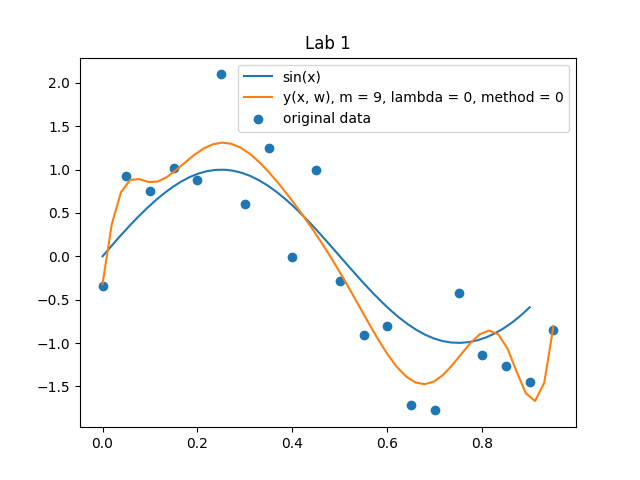
\includegraphics[width=\textwidth]{figures/Figure_6.png}
        \caption{$N = 20$时的拟合情况}
        \label{N20}
    \end{minipage}
\end{figure}

\begin{figure}[htbp]
    \begin{minipage}[t]{0.5\linewidth}
        \centering
        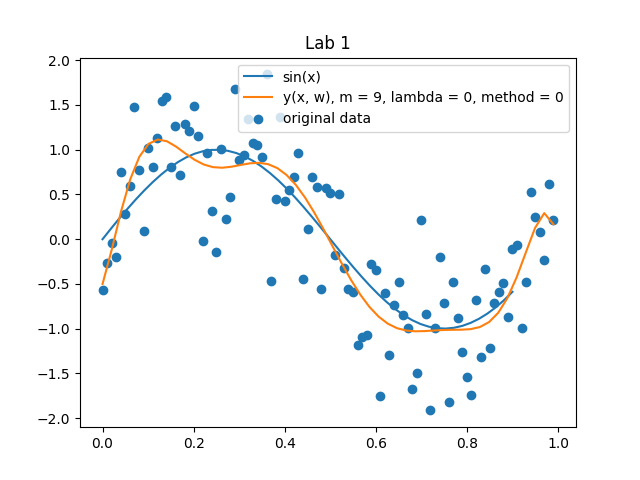
\includegraphics[width=\textwidth]{figures/Figure_7.png}
        \caption{$N = 100$时的拟合情况}
        \label{N100}
    \end{minipage}
    \begin{minipage}[t]{0.5\linewidth}
        \centering
        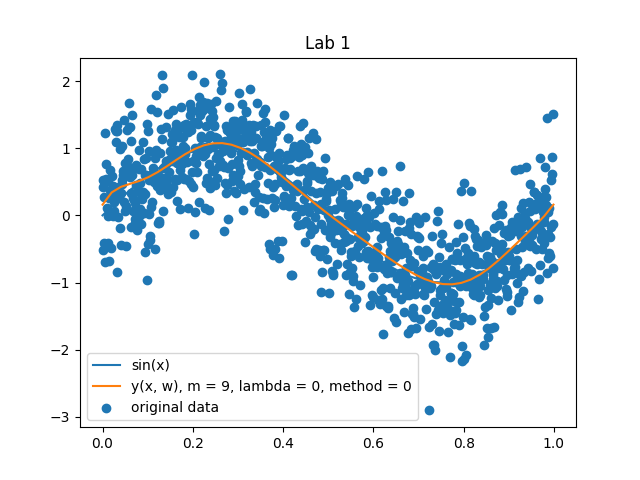
\includegraphics[width=\textwidth]{figures/Figure_8.png}
        \caption{$N = 1000$时的拟合情况}
        \label{N1000}
    \end{minipage}
\end{figure}

可以看到,随着样本数量逐渐增加,过拟合的现象有所解决。当样本数量$N = 1000$时,拟合的多项式函数已经非常接近于真实函数。

\subsection{有惩罚项}

\subsubsection{惩罚项系数的确定}

惩罚项系数$\lambda$可以由根均方(RMS)误差\cite{ref3}来确定,其中RMS的定义如式\eqref{rms}所示。

\begin{equation}
    E_{RMS} = \sqrt{\dfrac{2E(w^*)}{N}}
    \label{rms}
\end{equation}

多次调整$\lambda$,选取使得$E_{RMS}$最小的$\lambda$即可。

\subsubsection{仅调整多项式系数}

选取数据量$N = 10$,$\lambda = e^{-12}$,调整多项式系数,拟合情况如图\ref{m39}。

\begin{figure}[htbp]
    \centering
    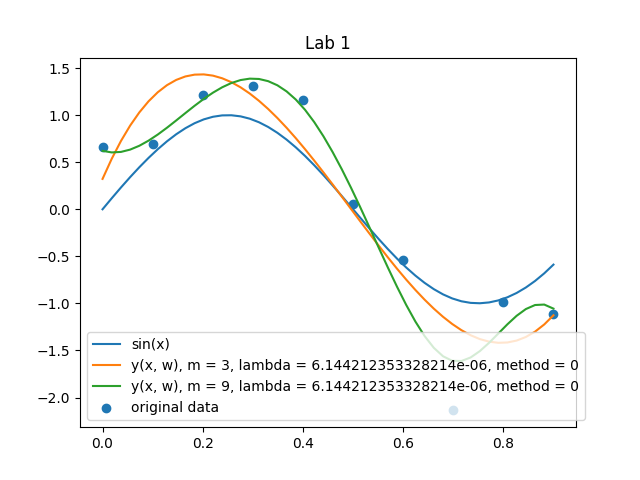
\includegraphics[width=0.7\textwidth]{figures/Figure_9.png}
    \caption{$m = 3, 9$时的拟合情况}
    \label{m39}
\end{figure}

可见$m = 9$时,原有的过拟合问题得到了很大程度上的缓解,甚至和$m = 3$时的拟合效果相似。

分析$m = 2, 3, 4, ... 9$时,训练数据和测试数据的误差,如图\ref{mn3},与图\ref{mn2}对比,可以发现通过添加惩罚项训练的多项式函数,对与新来的测试样本也能进行比较好的拟合,而误差不降反升的过拟合问题得到了很大程度的缓解。

\begin{figure}[htbp]
    \centering
    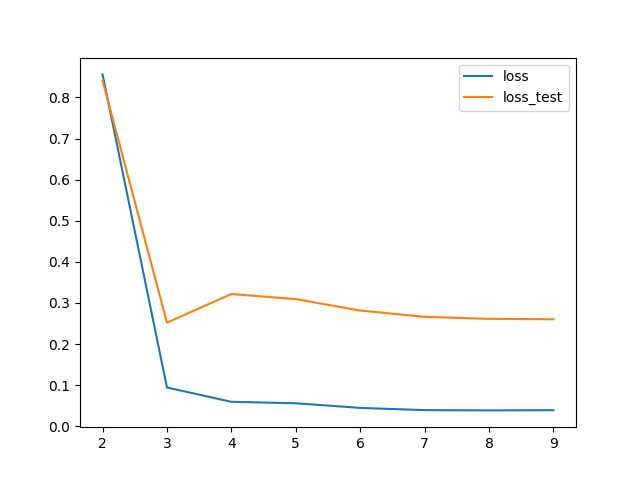
\includegraphics[width=0.7\textwidth]{figures/Figure_15.png}
    \caption{加添加惩罚项$\lambda$后,在$m = 2, 3, 4, ... 9$时,重新生成测试数据后,多项式函数拟合的误差}
    \label{mn3}
\end{figure}

\subsubsection{仅调整惩罚项系数}

调整惩罚项系数$\lambda$分别为$1, e^{-8}, e^{-50}, 0$,拟合情况如图\ref{lam}

\begin{figure}[htbp]
    \centering
    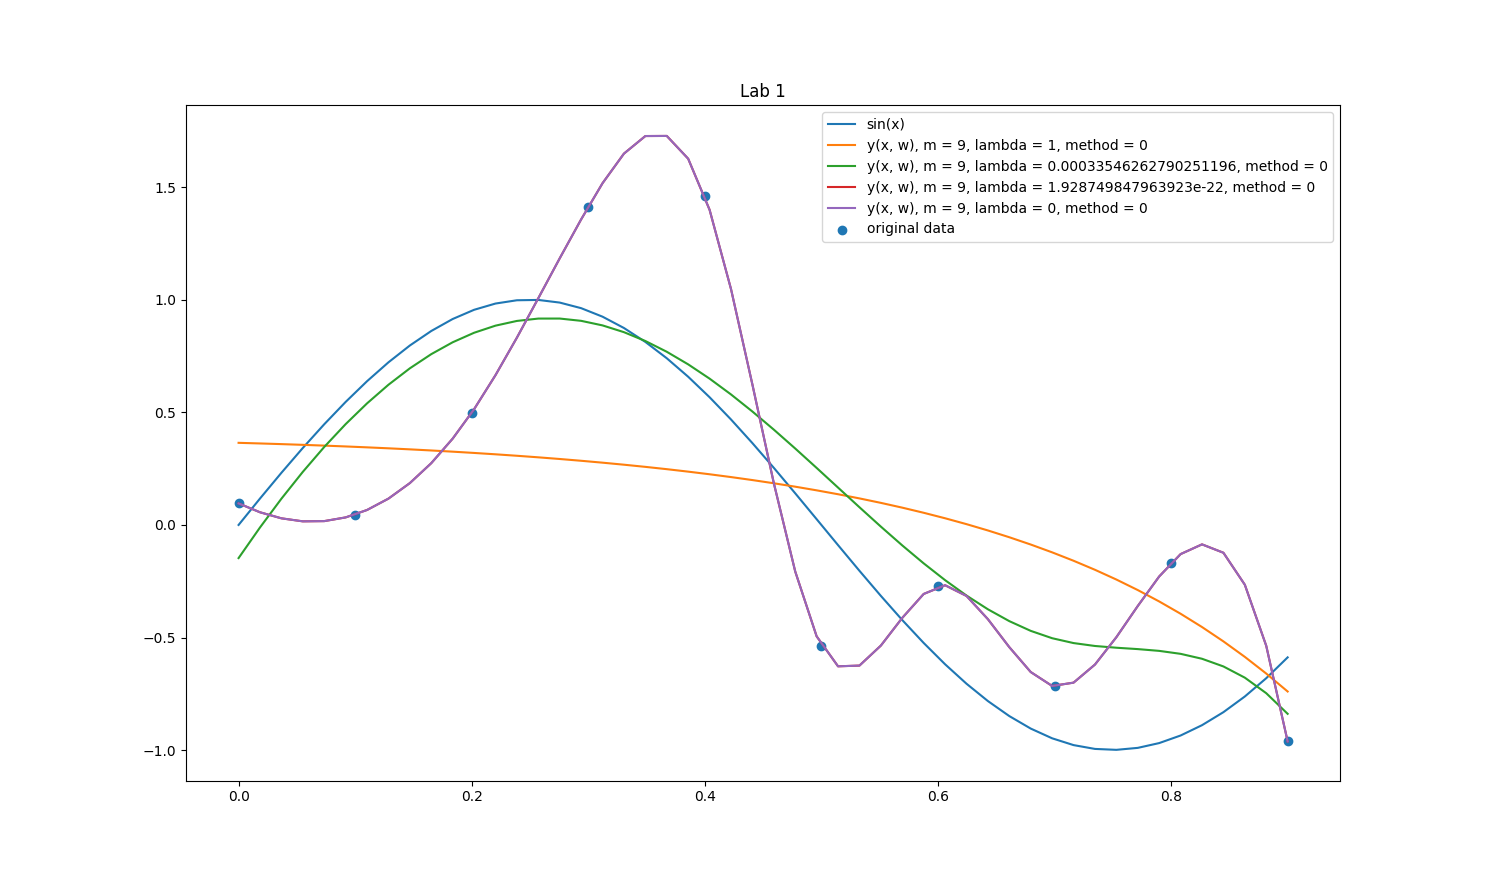
\includegraphics[width=0.7\textwidth]{figures/Figure_10.png}
    \caption{$\lambda = 1, e^{-8}, e^{-50}, 0$时的拟合情况}
    \label{lam}
\end{figure}

可以看到,当惩罚项过大(如$\lambda = 1$),或过小(如$\lambda = 0$)时,曲线拟合效果均不佳。所以选择一个合适的惩罚项系数将十分有利于曲线的拟合。

\subsubsection{附加研究}

测试$m = 50$,数据量$N = 100$时的解析解结果和共轭梯度方法得到的结果,如图\ref{m50}

\begin{figure}[htbp]
    \centering
    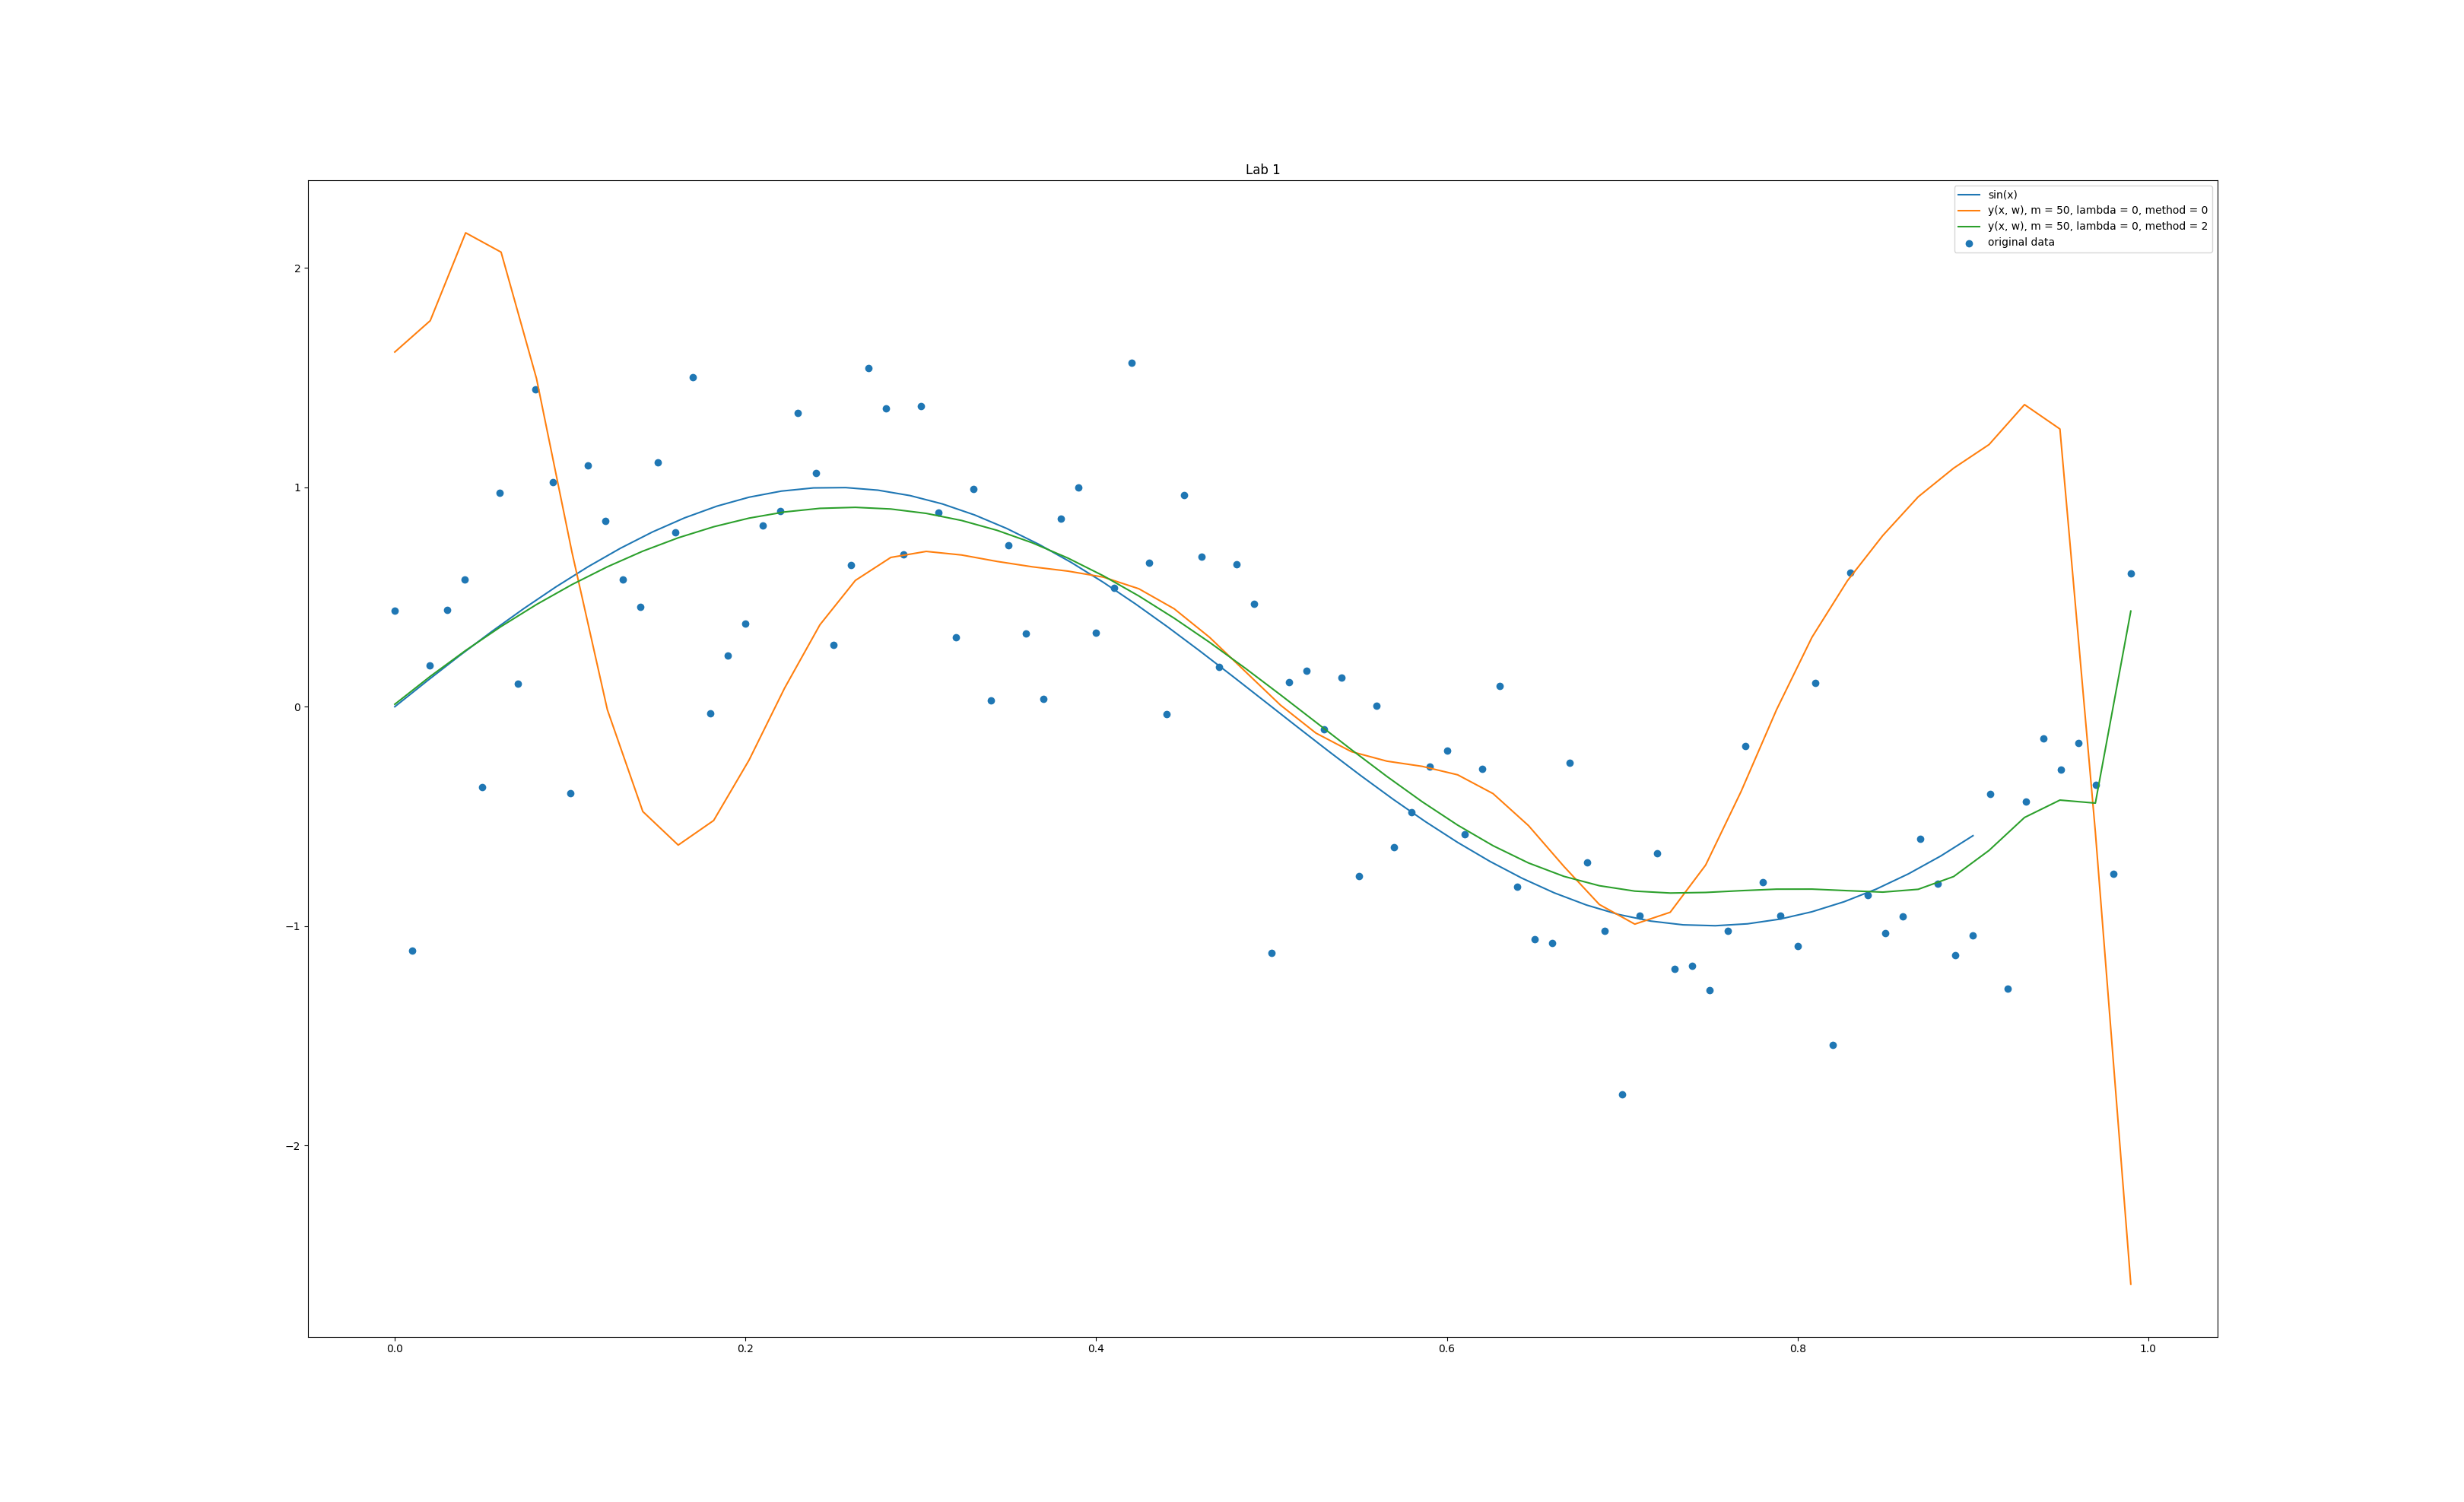
\includegraphics[width=0.7\textwidth]{figures/Figure_16.png}
    \caption{$m = 50$,数据量$N = 100$时的解析解结果和共轭梯度方法得到的结果}
    \label{m50}
\end{figure}

可见用解析解法拟合的曲线几乎完全丢失了$sin(2 \pi x)$的几何性质,而共轭梯度法拟合的曲线拟合程度极好。
